%% Figura 1 do exemplo do template — vista em corte longitudinal.
%% Desenho de exemplo, para ser substituído pelo desenho do seu pedido.
%% Regenerar com:  pdflatex figura-1-vista-em-corte.tex
%% Art. 39 — a figura é isenta de texto: só sinais de referência.
\documentclass[border=6pt]{standalone}
\usepackage{tikz}
\usetikzlibrary{patterns}
\begin{document}
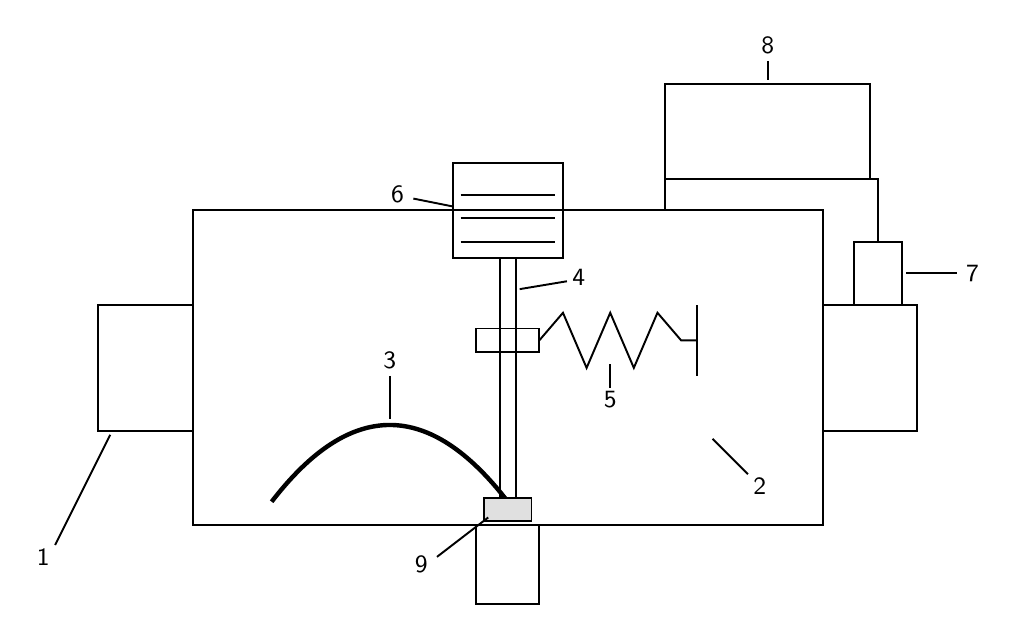
\begin{tikzpicture}[line width=0.7pt, font=\sffamily\small]
    % corpo tubular (2)
    \draw (0,0) rectangle (8,4);
    \draw (0,1.2) -- (-1.2,1.2) -- (-1.2,2.8) -- (0,2.8);      % bocal de entrada
    \draw (8,1.2) -- (9.2,1.2) -- (9.2,2.8) -- (8,2.8);        % bocal de saida
    \draw (3.6,0) -- (3.6,-1.0) -- (4.4,-1.0) -- (4.4,0);      % orificio de alivio
    % membrana elastica (3)
    \draw[line width=1.6pt] (1.0,0.3) .. controls (2.0,1.6) and (3.0,1.6) .. (4.0,0.3);
    % haste de acionamento (4) com ressalto de encosto
    \draw (3.9,0.3) rectangle (4.1,3.4);
    \draw (3.6,2.2) rectangle (4.4,2.5);
    % mola de retorno (5)
    \draw (4.4,2.35) -- (4.7,2.7) -- (5.0,2.0) -- (5.3,2.7) -- (5.6,2.0) -- (5.9,2.7) -- (6.2,2.35) -- (6.4,2.35);
    \draw (6.4,1.9) -- (6.4,2.8);
    % atuador eletromecanico (6)
    \draw (3.3,3.4) rectangle (4.7,4.6);
    \foreach \y in {3.6,3.9,4.2} \draw (3.4,\y) -- (4.6,\y);
    % sensor de pressao (7)
    \draw (8.4,2.8) rectangle (9.0,3.6);
    % unidade de controle (8)
    \draw (6.0,4.4) rectangle (8.6,5.6);
    \draw (4.7,4.0) -- (6.0,4.0) -- (6.0,4.4);
    \draw (8.7,3.6) -- (8.7,4.4) -- (8.6,4.4);
    % assento de vedacao de dupla face (9)
    \draw[fill=black!12] (3.7,0.05) rectangle (4.3,0.35);
    % sinais de referencia
    % (1) e o conjunto inteiro: a linha de chamada aponta o contorno do
    % dispositivo, nao um componente. Sem este sinal, o (1) citado no relatorio,
    % nas reivindicacoes e no resumo nao teria correspondencia em figura alguma
    % (art. 27, VI e art. 39, IV).
    \node at (-1.9,-0.4) {1};  \draw (-1.75,-0.25) -- (-1.05,1.15);
    \node at (7.2,0.5)  {2};   \draw (7.05,0.65) -- (6.6,1.1);
    \node at (2.5,2.1)  {3};   \draw (2.5,1.9) -- (2.5,1.35);
    \node at (4.9,3.15) {4};   \draw (4.75,3.1) -- (4.15,3.0);
    \node at (5.3,1.6)  {5};   \draw (5.3,1.75) -- (5.3,2.05);
    \node at (2.6,4.2)  {6};   \draw (2.8,4.15) -- (3.3,4.05);
    \node at (9.9,3.2)  {7};   \draw (9.7,3.2) -- (9.05,3.2);
    \node at (7.3,6.1)  {8};   \draw (7.3,5.9) -- (7.3,5.65);
    \node at (2.9,-0.5) {9};   \draw (3.1,-0.4) -- (3.75,0.1);
\end{tikzpicture}
\end{document}
